TODO

\subsection{Evaluation of Supervised Learning Surrogates}
\label{sec:modelres}

We begin by evaluating a diverse set of surrogate classes that we proposed
earlier. In particular, we aim to study considered models in terms of regression
performance and evaluation complexity.
Following~\cref{sec:experiment-methodology}, where we proposed four experiments
that accomplish this task, we present and discuss our results in the next
several sections.


\subsubsection{Hyperparameter Tuning}

The first two experiments perform Bayesian optimisation to maximise~$R^2$ in
cross-validated setting as a function of model hyperparameters. While in the
first experiment we limit training and testing sets to the scope of four slices of the
feature space, in the second experiment we lift this restriction.

The results displayed in~\cref{fig:exp1-time-vs-reg} indicate that in the first
experiment, gradient boosted trees clearly appear to be the most accurate as
well as the fastest surrogate class in terms of mean prediction time. Following
that, we note that extremely randomised trees, support vector machines and
artificial neural networks also achieved satisfactory results with respect to both examined metrics.
While the remainder of tested surrogate classes does not exhibit problems in
complexity, its regression performance falls below average.

\begin{figure}[h]
	\centering
	\begin{subfigure}[b]{0.333\textwidth}
		\centering
		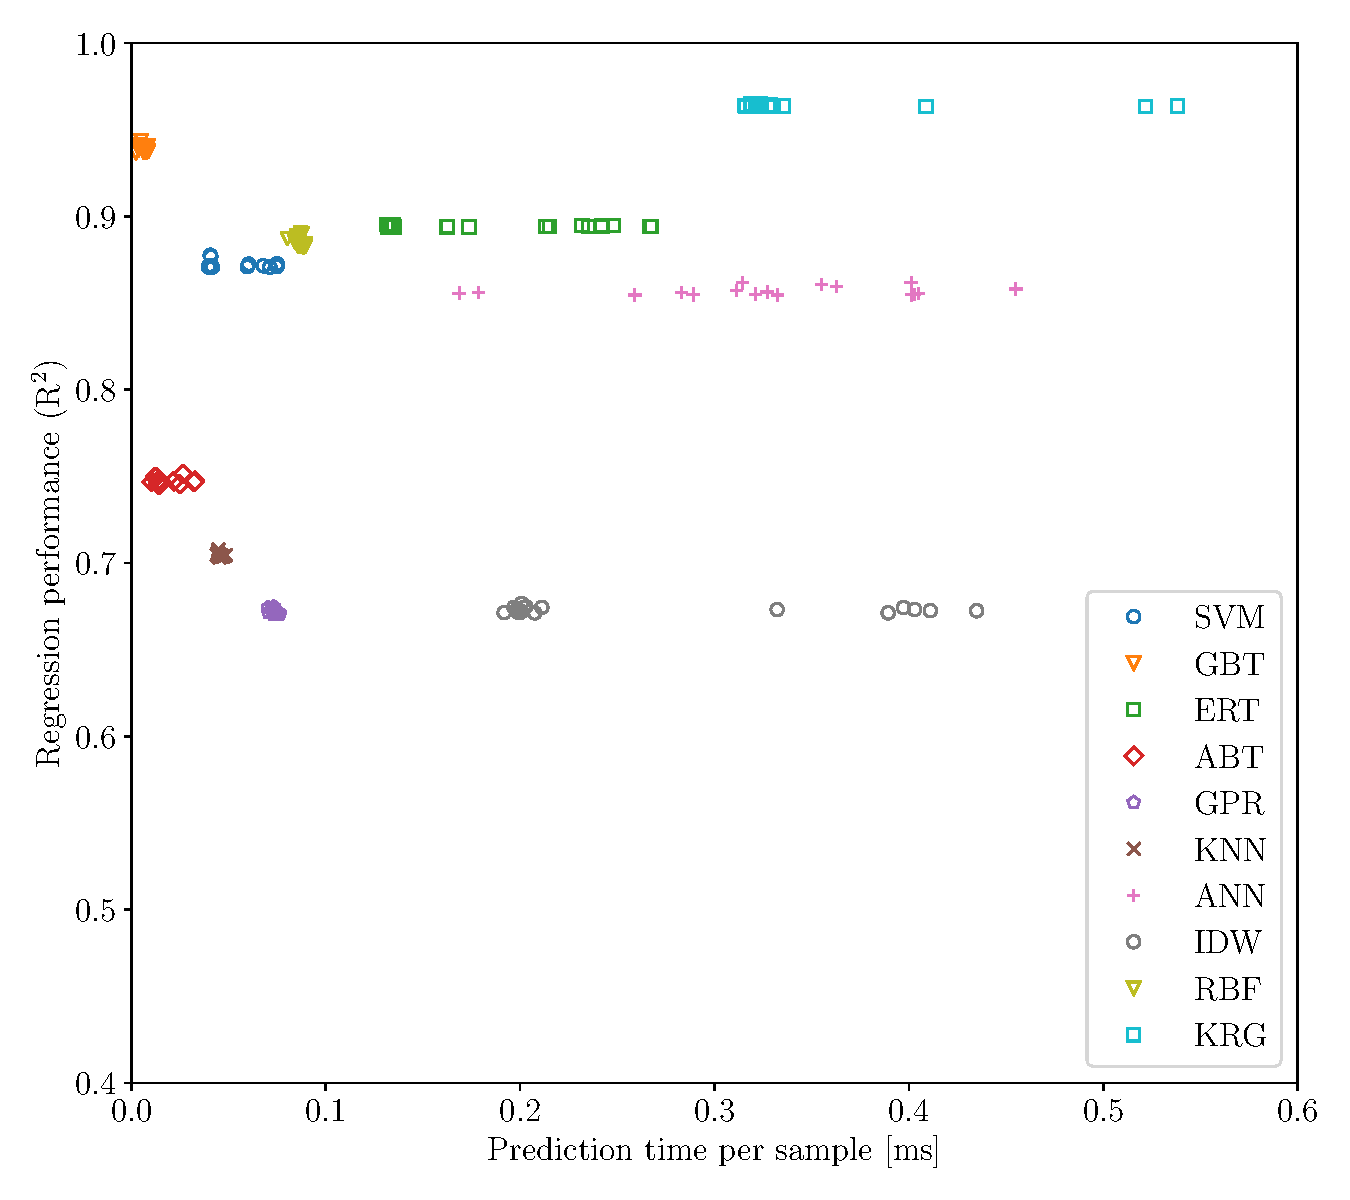
\includegraphics[width=\linewidth]{exp1_slice0}
		% TODO: only a placeholder, regenerate when data becomes available
		\caption{Run 2, batches 0-3}
	\end{subfigure}\hfill%
	\begin{subfigure}[b]{0.333\textwidth}
		\centering
		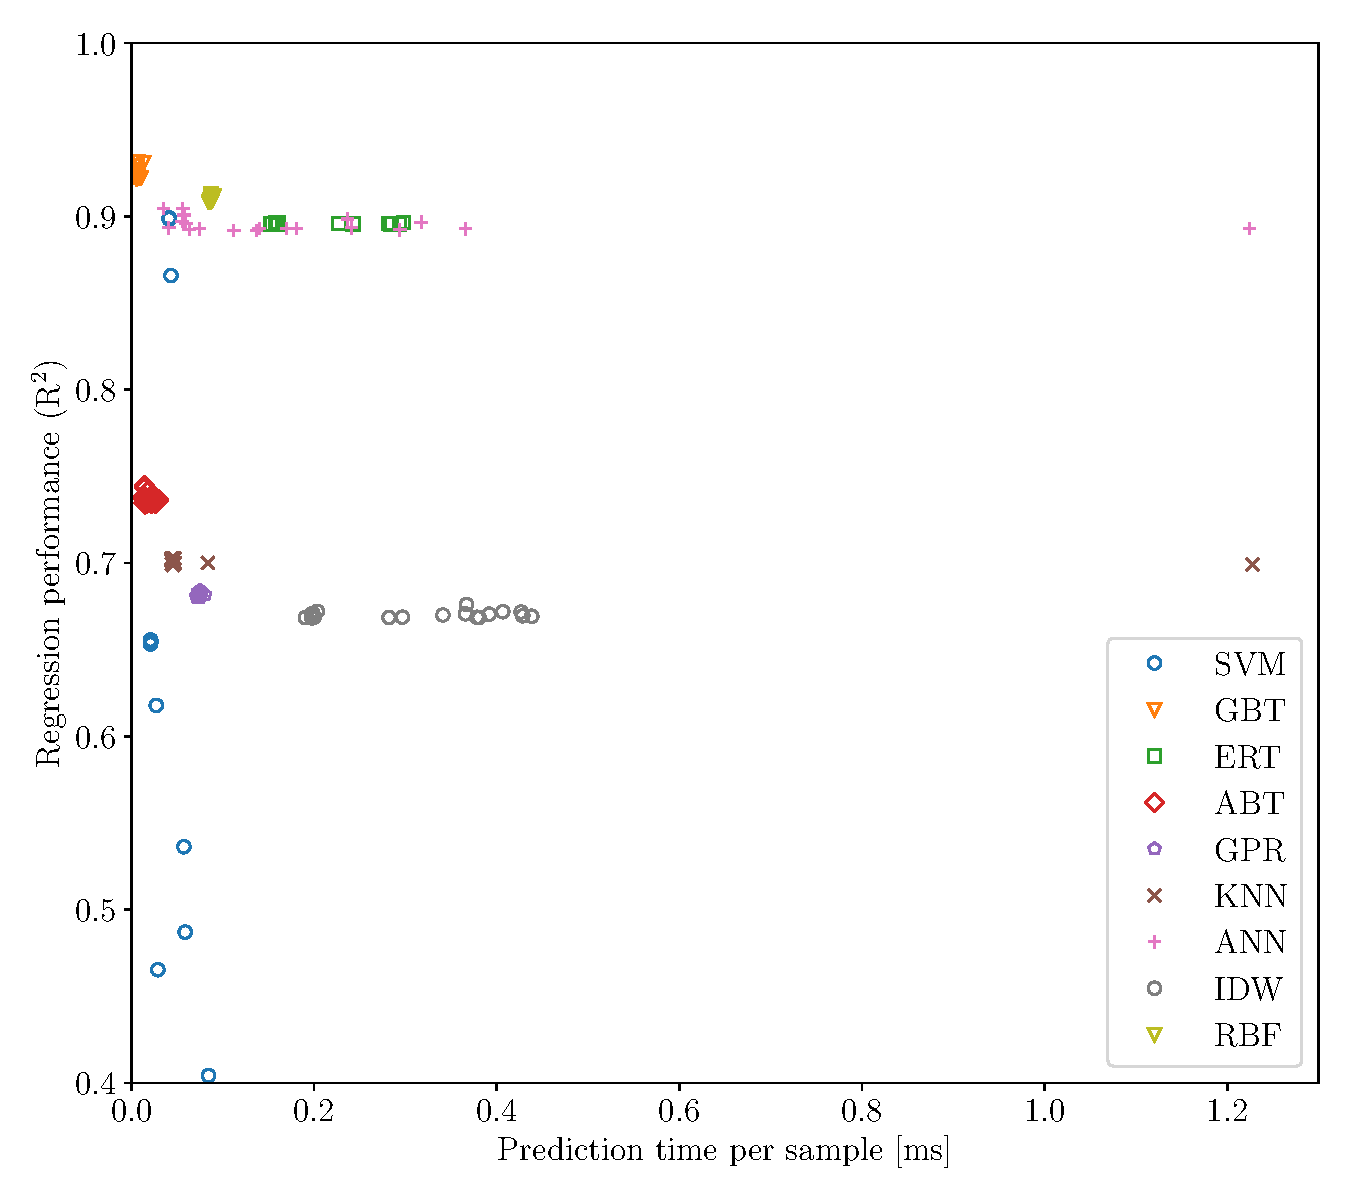
\includegraphics[width=\linewidth]{exp1_slice1}
		% TODO: only a placeholder, regenerate when data becomes available
		\caption{Run 2, batches 100-103}
	\end{subfigure}\hfill%
	\begin{subfigure}[b]{0.333\textwidth}
		\centering
		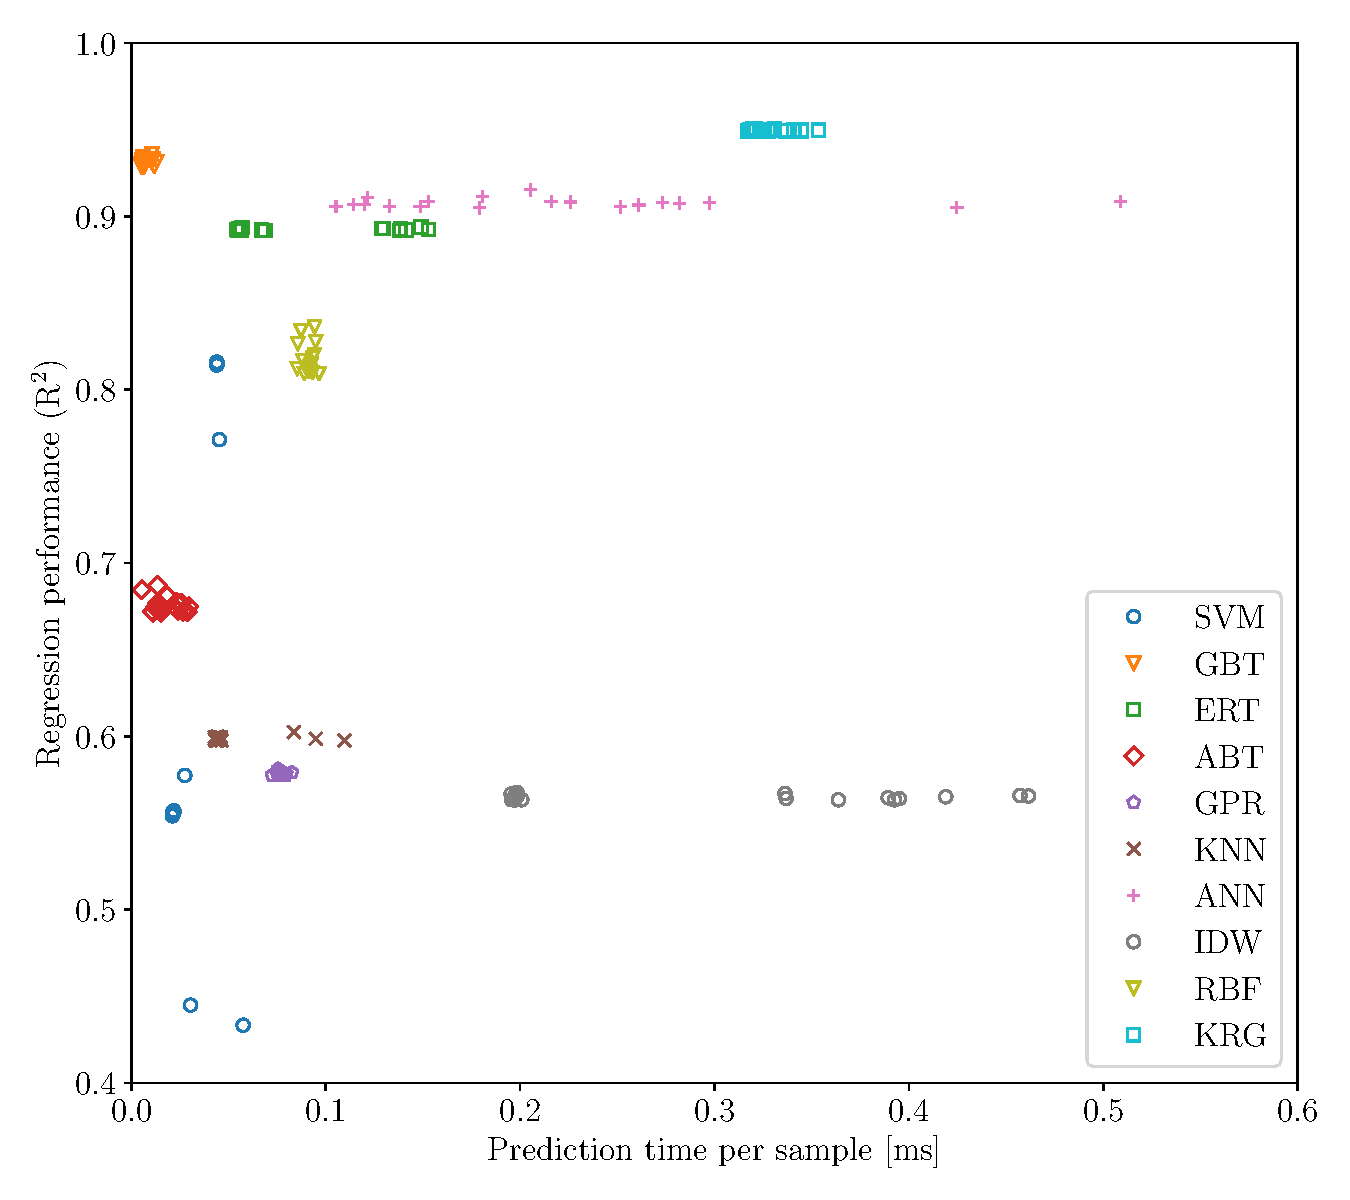
\includegraphics[width=\linewidth]{exp1_slice2}
		% TODO: only a placeholder, regenerate when data becomes available
		\caption{Run 2, batches 200-203}
	\end{subfigure}
	\caption{20~best-performing surrogates per each considered class, plotted in
		terms of complexity (as $\overline{t}_{\text{pred.}}$) and regression
		performance (as~$R^2$) on selected slices of run~2, evaluated in experiment~1.}
	\label{fig:exp1-time-vs-reg}
\end{figure}

% TODO: add table here or in appendix with hard numbers, for each class take 20
% best performing models from each slice, concatenate and calculate mean and std
% for each metric

% TODO: do the same thing for the second experiment
\newpage
\begin{wrapfigure}{r}{0.333\textwidth}
	\centering
	\vspace{-3ex}
	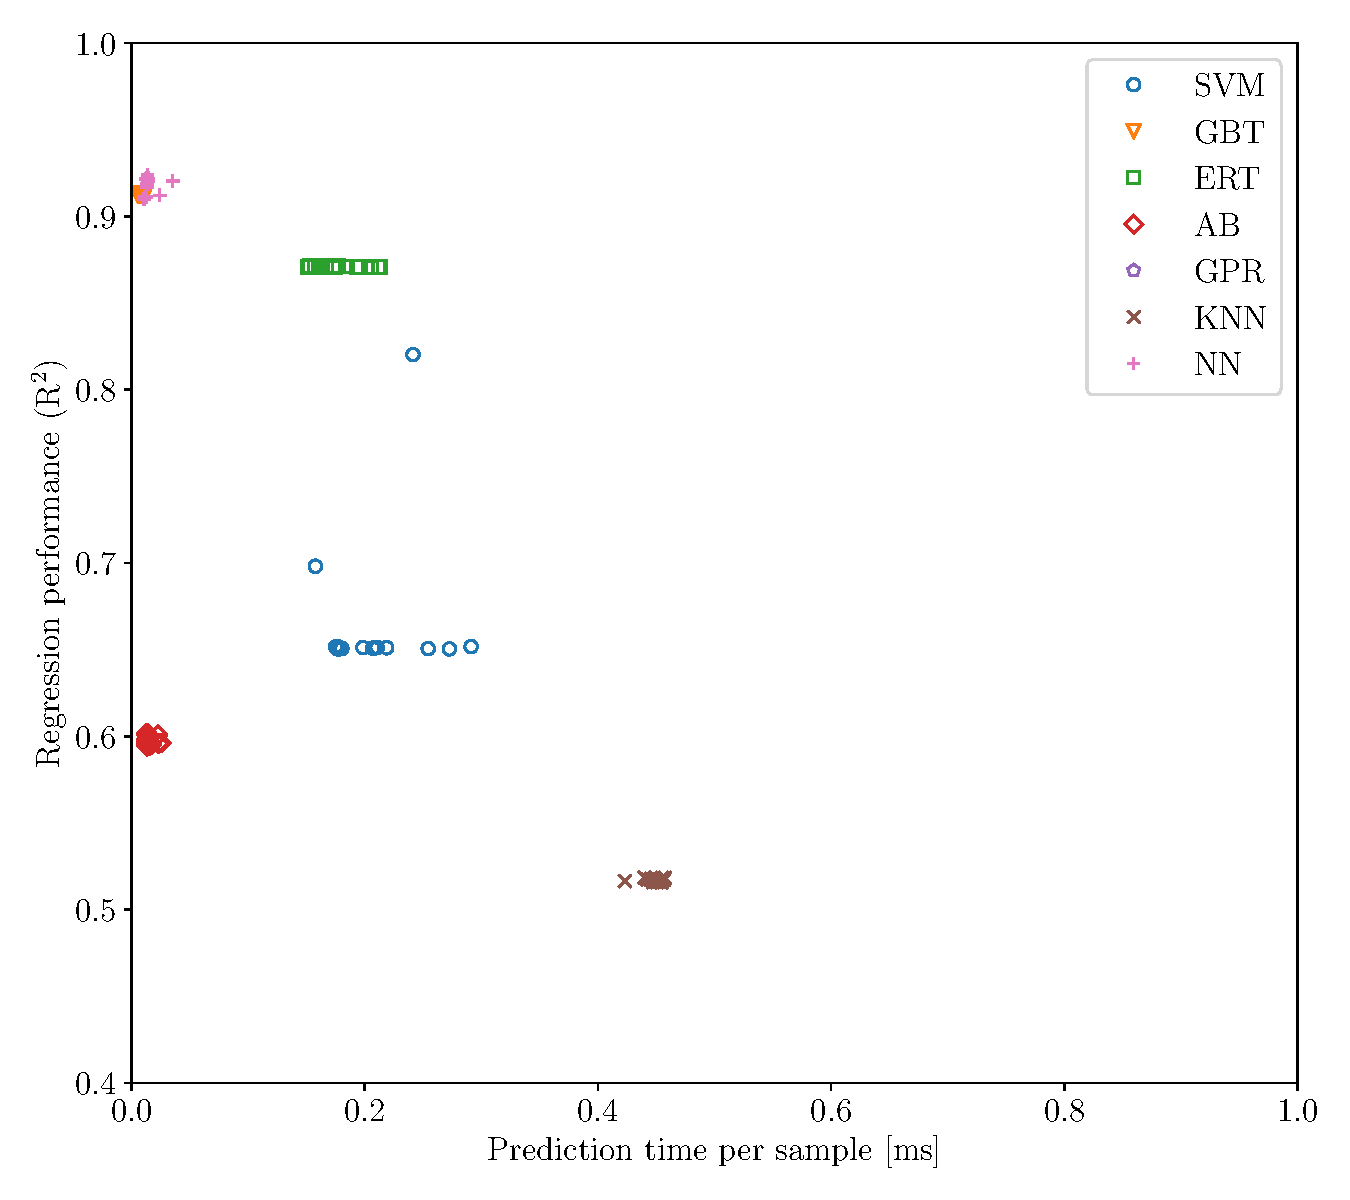
\includegraphics[width=\linewidth]{exp2_time_vs_reg}
	% TODO: only a placeholder, regenerate when data becomes available
	\caption{Results of experiment~2, plotted analogously
	to~\cref{fig:exp1-time-vs-reg}.}
	\label{fig:exp2-time-vs-reg}
	\vspace{-4ex}
\end{wrapfigure}

% TODO: multislice description
TODO: multislice description

\subsubsection{Scaling Benchmark}

In the next experiment we examine surrogate scaling properties correlating
metrics of interest with progressively increasing training set size. The results
shown in~\cref{fig:scaling} seem to suggest that in terms of regression performance,
methods based on decision trees and artificial neural networks offer the best accuracy on
larger sets overall. This is a curious extension of the previous findings, where
gradient boosted trees were observed to significantly dominate over the rest of
the examined methods. With increasing training set size, their relative advantage is
clearly gradually diminished.

\begin{figure}[h]
	\centering
	\begin{subfigure}[b]{0.333\textwidth}
		\centering
		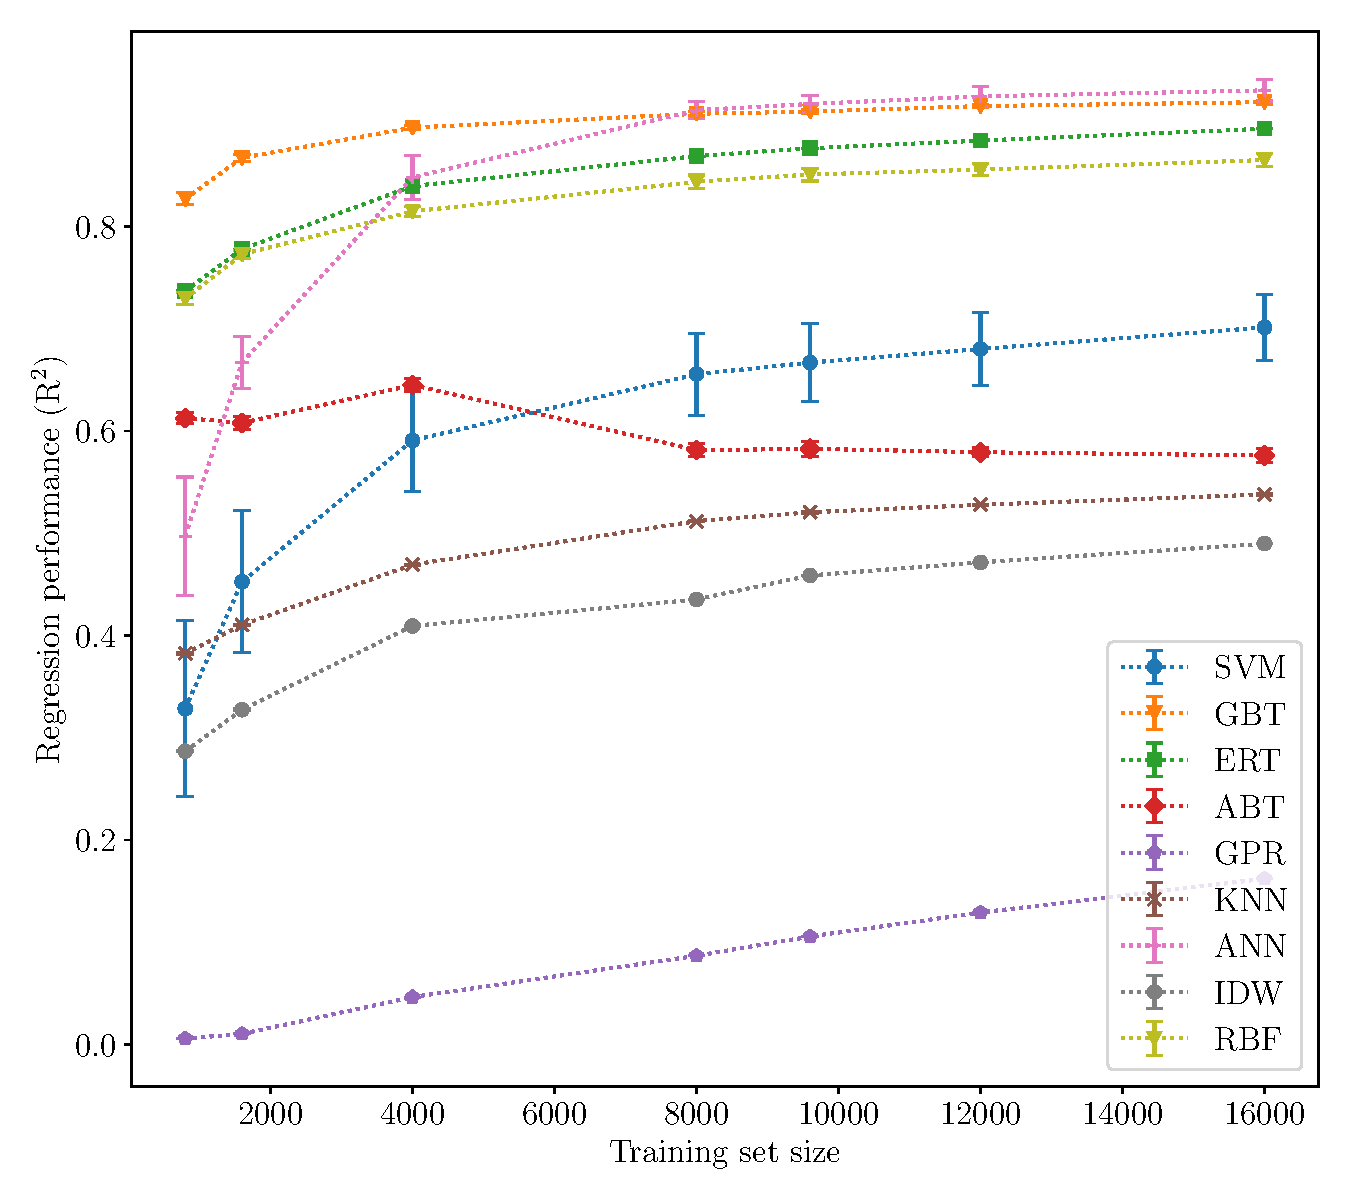
\includegraphics[width=\linewidth]{scaling_metric_r2}
		% TODO: only a placeholder, regenerate when data becomes available
		\caption{Regression performance (as $R^2$)}
	\end{subfigure}\hfill%
	\begin{subfigure}[b]{0.333\textwidth}
		\centering
		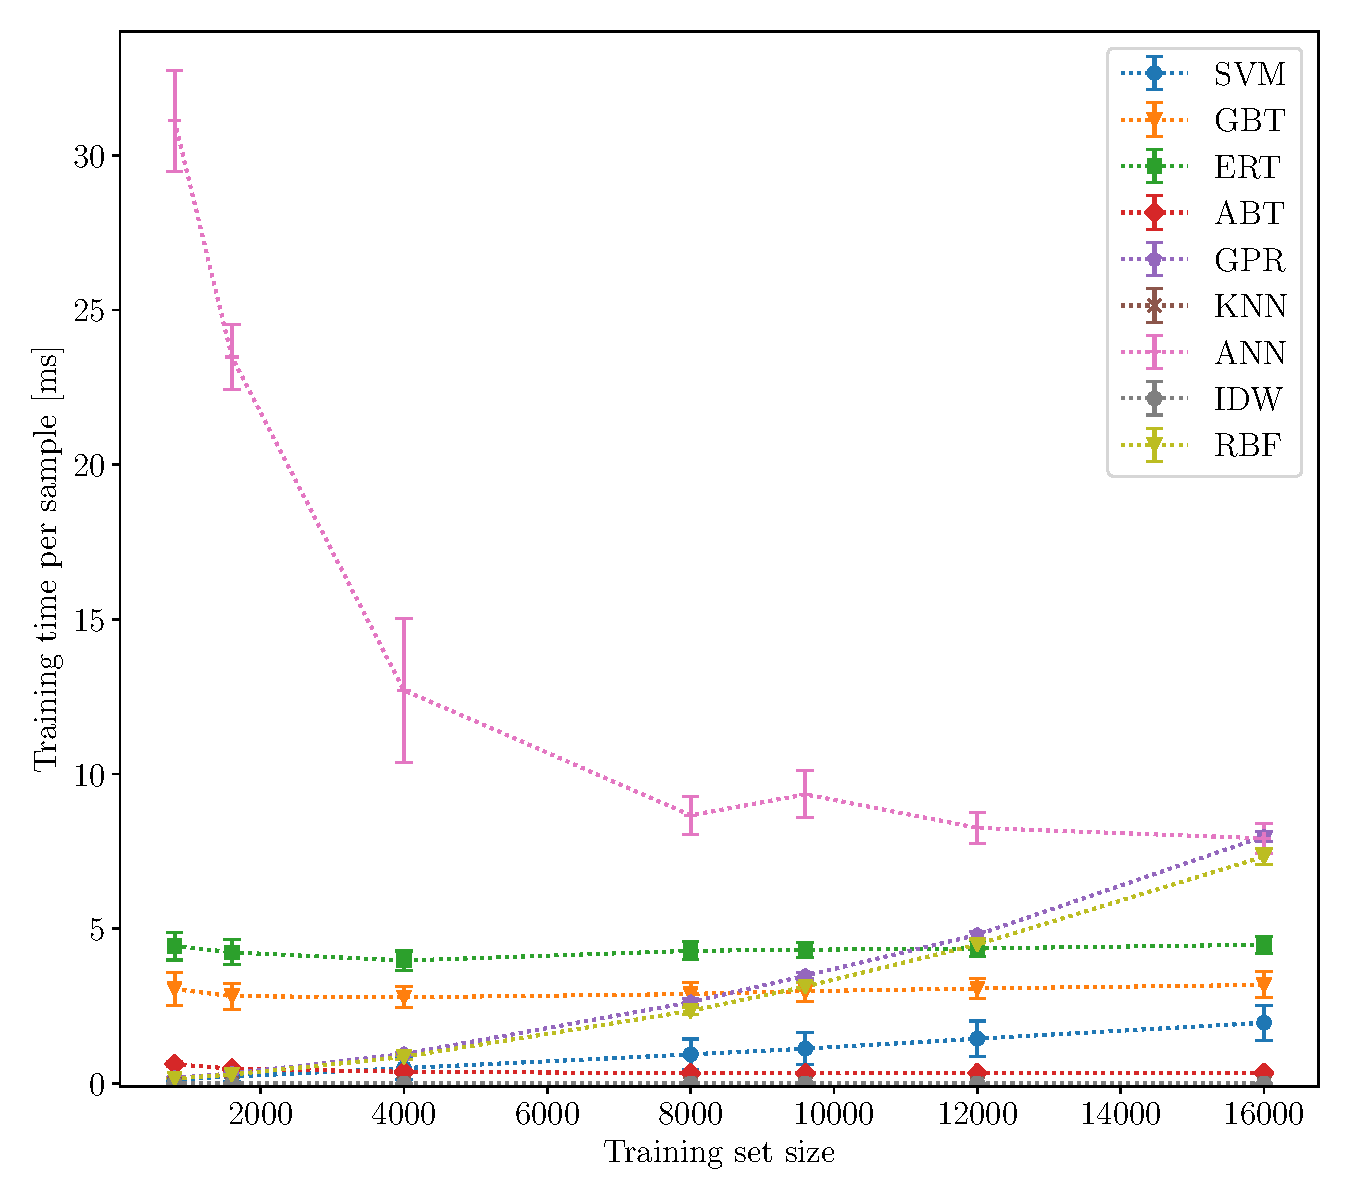
\includegraphics[width=\linewidth]{scaling_time_train}
		% TODO: only a placeholder, regenerate when data becomes available
		\caption{Complexity (as~$\overline{t}_{\text{trn.}}$)}
	\end{subfigure}\hfill%
	\begin{subfigure}[b]{0.333\textwidth}
		\centering
		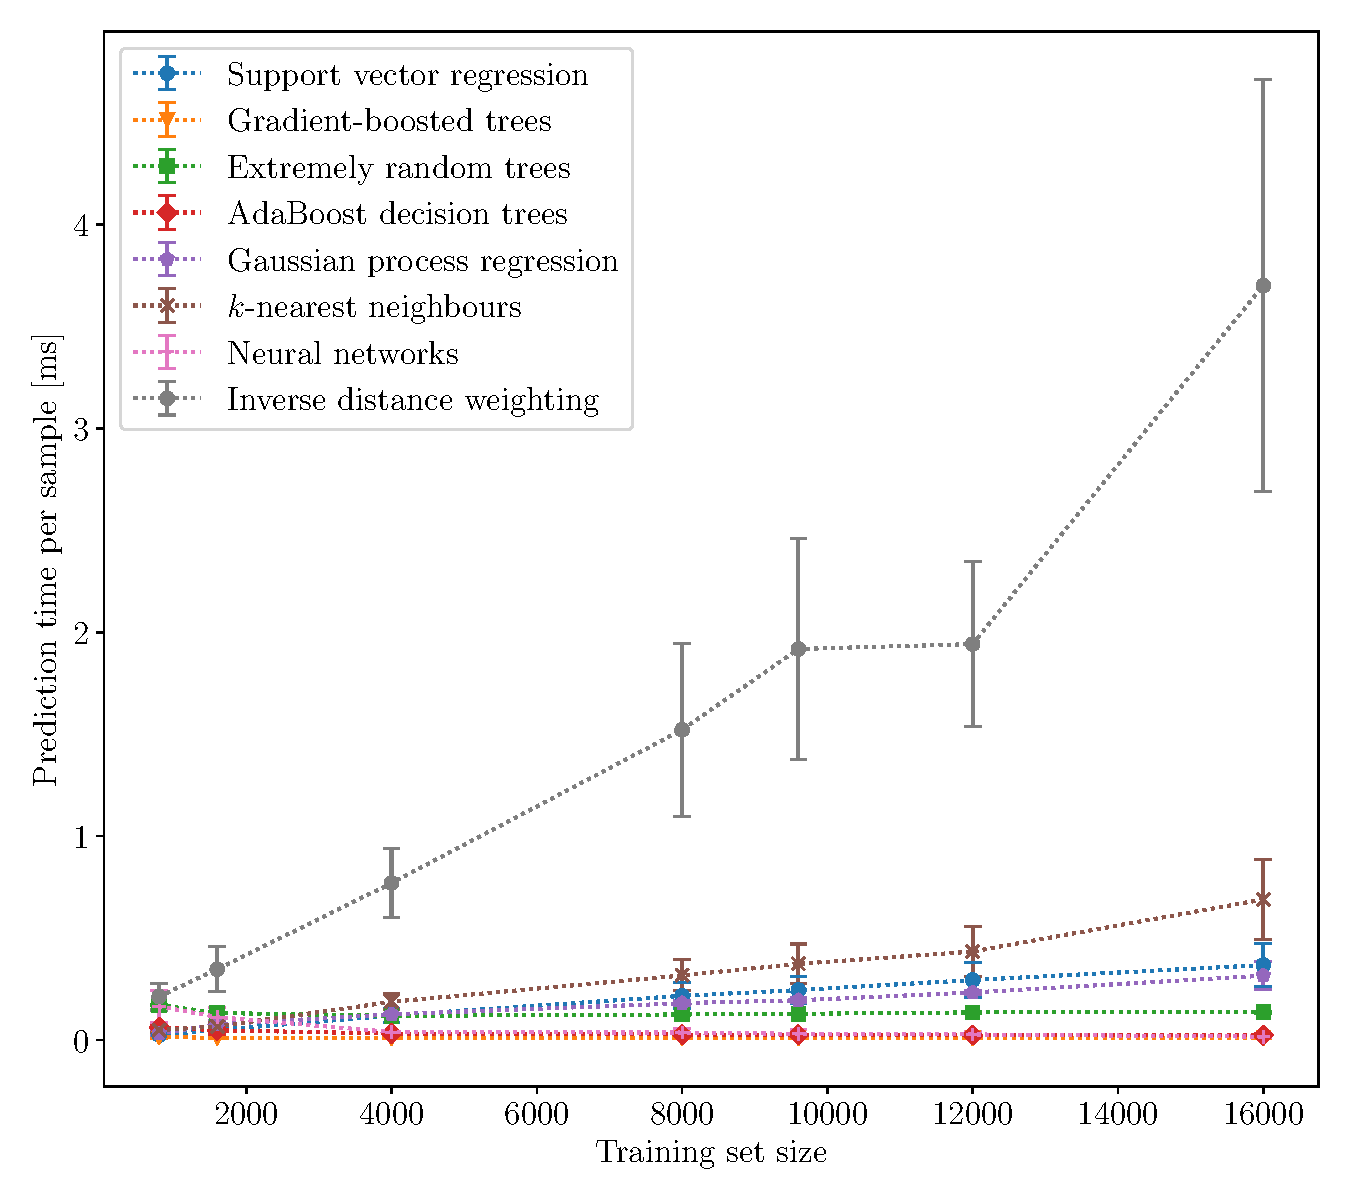
\includegraphics[width=\linewidth]{scaling_time_pred}
		% TODO: only a placeholder, regenerate when data becomes available
		\caption{Complexity (as~$\overline{t}_{\text{pred.}}$)}
	\end{subfigure}
	\caption{Various metrics collected during experiment 3 (scaling
	benchmark) displayed as a function of training set size.}
	\label{fig:scaling}
\end{figure}

According to our experiment, the lowest mean training time is generally achieved
by instance-based learning methods, which seem to offer near-constant scaling
characteristics at the expense of significant performance increase later during
prediction. Following that, we observe that the majority of tree-based methods also exhibit
desirable properties. The notable exception here appear to be artificial neural networks,
which are the only model to utilise parallelisation. As such, their constant
synchronisation overhead presumably hinders performance on small training sets,
producing misleading results when divided by the number of samples.

In terms of mean prediction time, all tested surrogates except previously mentioned
instance-based learning methods scale exceptionally well. Tree-based generally
models appear to perform the fastest.

% TODO: add tables here or in appendix with scaling results; for each metric
% create a table with rows = classes, columns = training set size, cells = mean +/- std
% it may be a lot, decide on placement and layout!


\subsubsection{Competitive Surrogate Training}

TODO

\begin{figure}[h]
	\centering
	\begin{subfigure}[b]{0.25\textwidth}
		\centering
		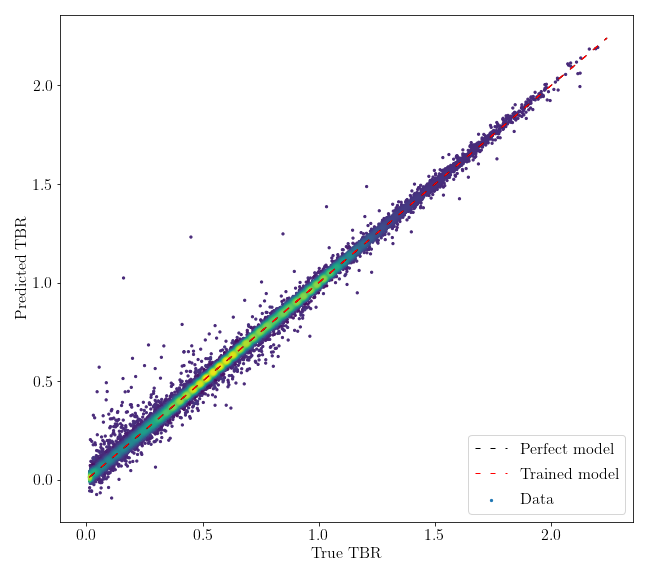
\includegraphics[width=\linewidth]{run1_5ke_1h3f128_4974_performance}
		% TODO: only a placeholder, regenerate when data becomes available
	\end{subfigure}\hfill%
	\begin{subfigure}[b]{0.25\textwidth}
		\centering
		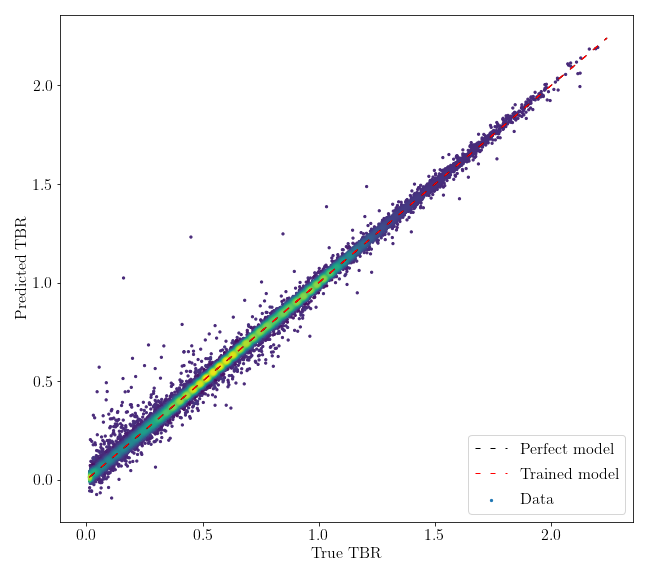
\includegraphics[width=\linewidth]{run1_5ke_1h3f128_4974_performance}
		% TODO: only a placeholder, regenerate when data becomes available
	\end{subfigure}\hfill%
	\begin{subfigure}[b]{0.25\textwidth}
		\centering
		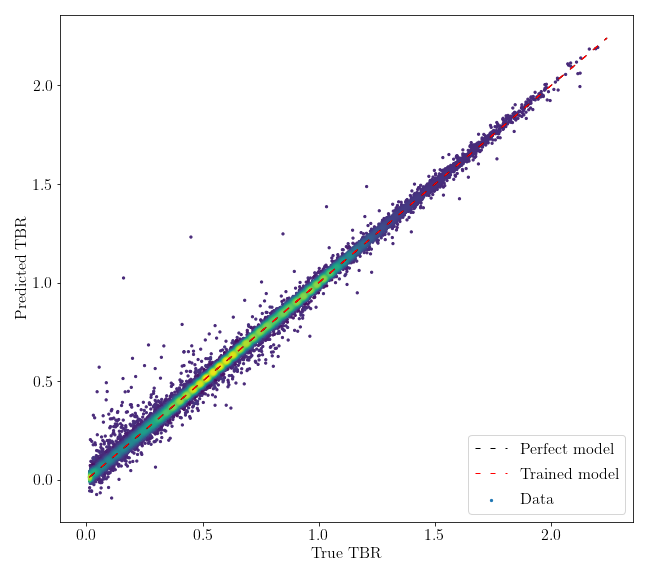
\includegraphics[width=\linewidth]{run1_5ke_1h3f128_4974_performance}
		% TODO: only a placeholder, regenerate when data becomes available
	\end{subfigure}\hfill%
	\begin{subfigure}[b]{0.25\textwidth}
		\centering
		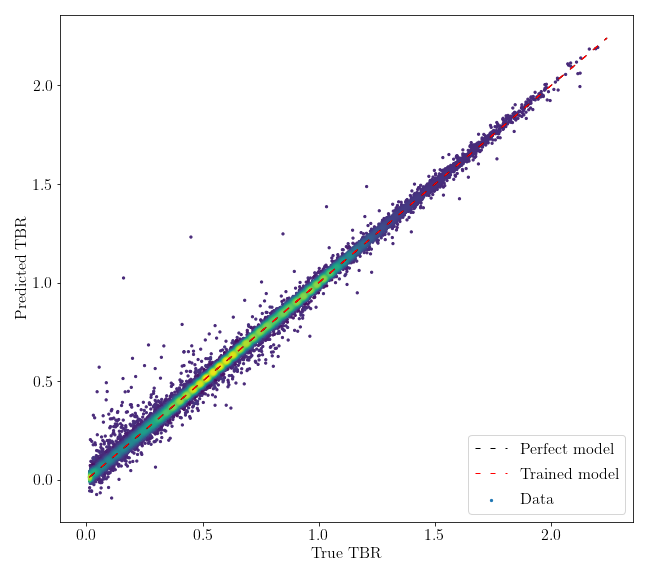
\includegraphics[width=\linewidth]{run1_5ke_1h3f128_4974_performance}
		% TODO: only a placeholder, regenerate when data becomes available
	\end{subfigure}

	\begin{subfigure}[b]{0.25\textwidth}
		\centering
		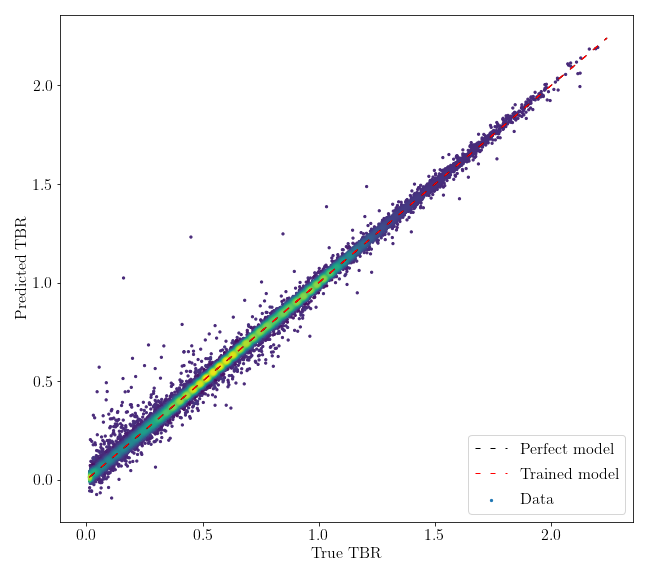
\includegraphics[width=\linewidth]{run1_5ke_1h3f128_4974_performance}
		% TODO: only a placeholder, regenerate when data becomes available
	\end{subfigure}\hfill%
	\begin{subfigure}[b]{0.25\textwidth}
		\centering
		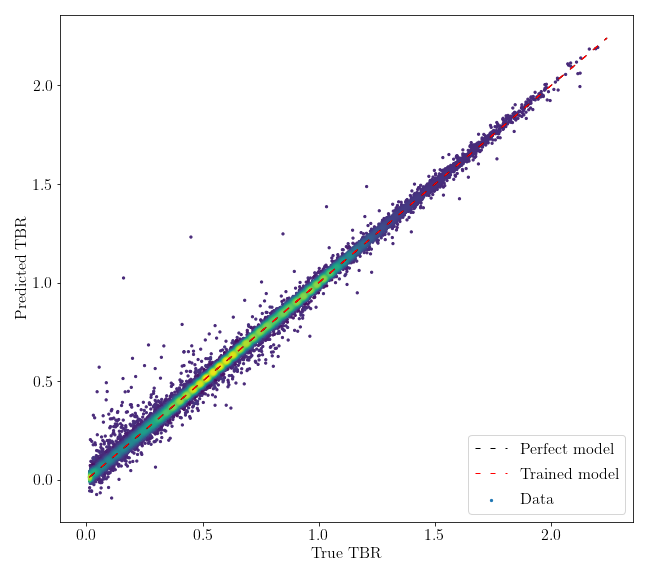
\includegraphics[width=\linewidth]{run1_5ke_1h3f128_4974_performance}
		% TODO: only a placeholder, regenerate when data becomes available
	\end{subfigure}\hfill%
	\begin{subfigure}[b]{0.25\textwidth}
		\centering
		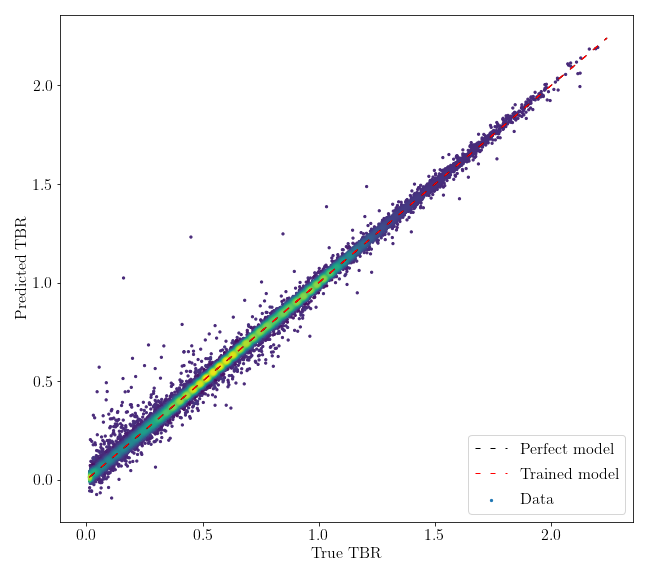
\includegraphics[width=\linewidth]{run1_5ke_1h3f128_4974_performance}
		% TODO: only a placeholder, regenerate when data becomes available
	\end{subfigure}\hfill%
	\begin{subfigure}[b]{0.25\textwidth}
		\centering
		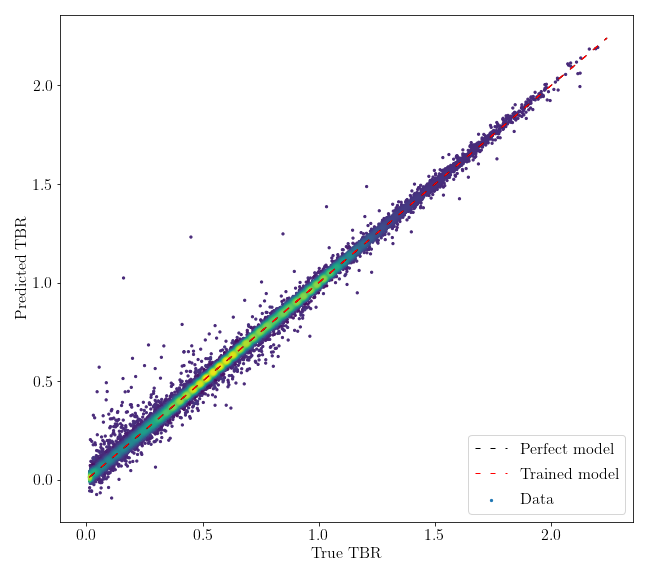
\includegraphics[width=\linewidth]{run1_5ke_1h3f128_4974_performance}
		% TODO: only a placeholder, regenerate when data becomes available
	\end{subfigure}
	\caption{Regression performance of models 1-4 (row 1, from the left) and 5-8
		(row 2) trained in experiment~4 (competitive surrogate training), viewed
		as true vs. predicted TBR on a test set of a selected cross-validation
		fold. Due to large set sizes, points are randomly subsampled and coloured by density.}
	\label{fig:reg-performance}
\end{figure}

\newpage

\begin{wrapfigure}{r}{0.4\textwidth}
  \vspace{-60pt}
  \begin{center}
    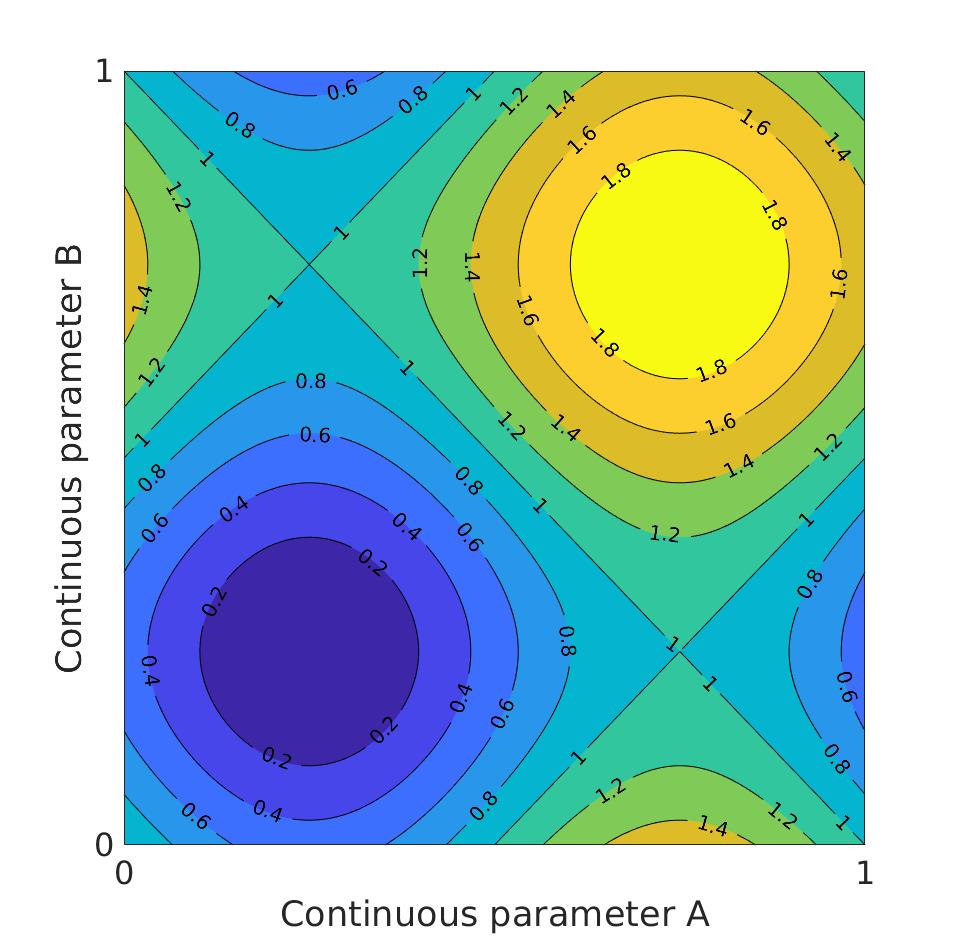
\includegraphics[width=0.4\textwidth]{fig5_sintoy.jpg}
	\caption{Sinusoidal toy TBR theory over two continuous parameters, wavenumber 1}
    \label{fig:sintoy}
  \end{center}
  \vspace{-10pt}
\end{wrapfigure}

\subsection{Results of Adaptive Sampling}
\label{sec:adaptiveres}

In order to test our QASS prototype, several functional toy theories for TBR were developed as alternatives to the expensive MC model. By far the most robust of these was the following sinusoidal theory with adjustable wavenumber parameter $n$:

\begin{equation}
	\text{TBR} = \text{Mean}_{i \in C} \left[ \frac{1 + \sin(2\pi n (x_i - 1/2)) }{2} \right]
\end{equation}

plotted in~\cref{fig:sintoy} for $n=1$ and two continuous parameters $C$. ANNs
trained on this model demonstrated similar performance to those on the expensive
MC model. QASS performance was verified by training a $\text{1h3f}(256)$ ANN on
the sinusoidal theory for varied quantities of initial, incremental, and MCMC
candidate samples. Although the scope of this project did not include thorough
searches of this hyperparameter domain, sufficient runs were made to identify
some likely trends.

An increase in MCMC candidate samples was seen to have a positive but very weak
effect on final surrogate precision, suggesting that the runtime of MCMC on each
iteration can be limited for increased efficiency. -- Awaiting test results on
initial sample quantity --. The most complex dynamics arose with the adjustment
of sample increment, shown in~\cref{fig:qassincr}. For each tested initial sample quantity N, the optimal number of step samples was seen to be well-approximated by $\sqrt{N}$; the plotted error trends suggest that incremental samples larger than this optimum give slower model improvement on both the training and evaluation sets, and a larger minimum error on the evaluation set. This performance distinction is predicted to be even more significant when trained on the expensive MC model, where the number of sample evaluations will serve as the primary bottleneck for computation time.
\begin{figure}[h!]
    \centering
    \begin{subfigure}[t]{0.5\textwidth}
        \centering
        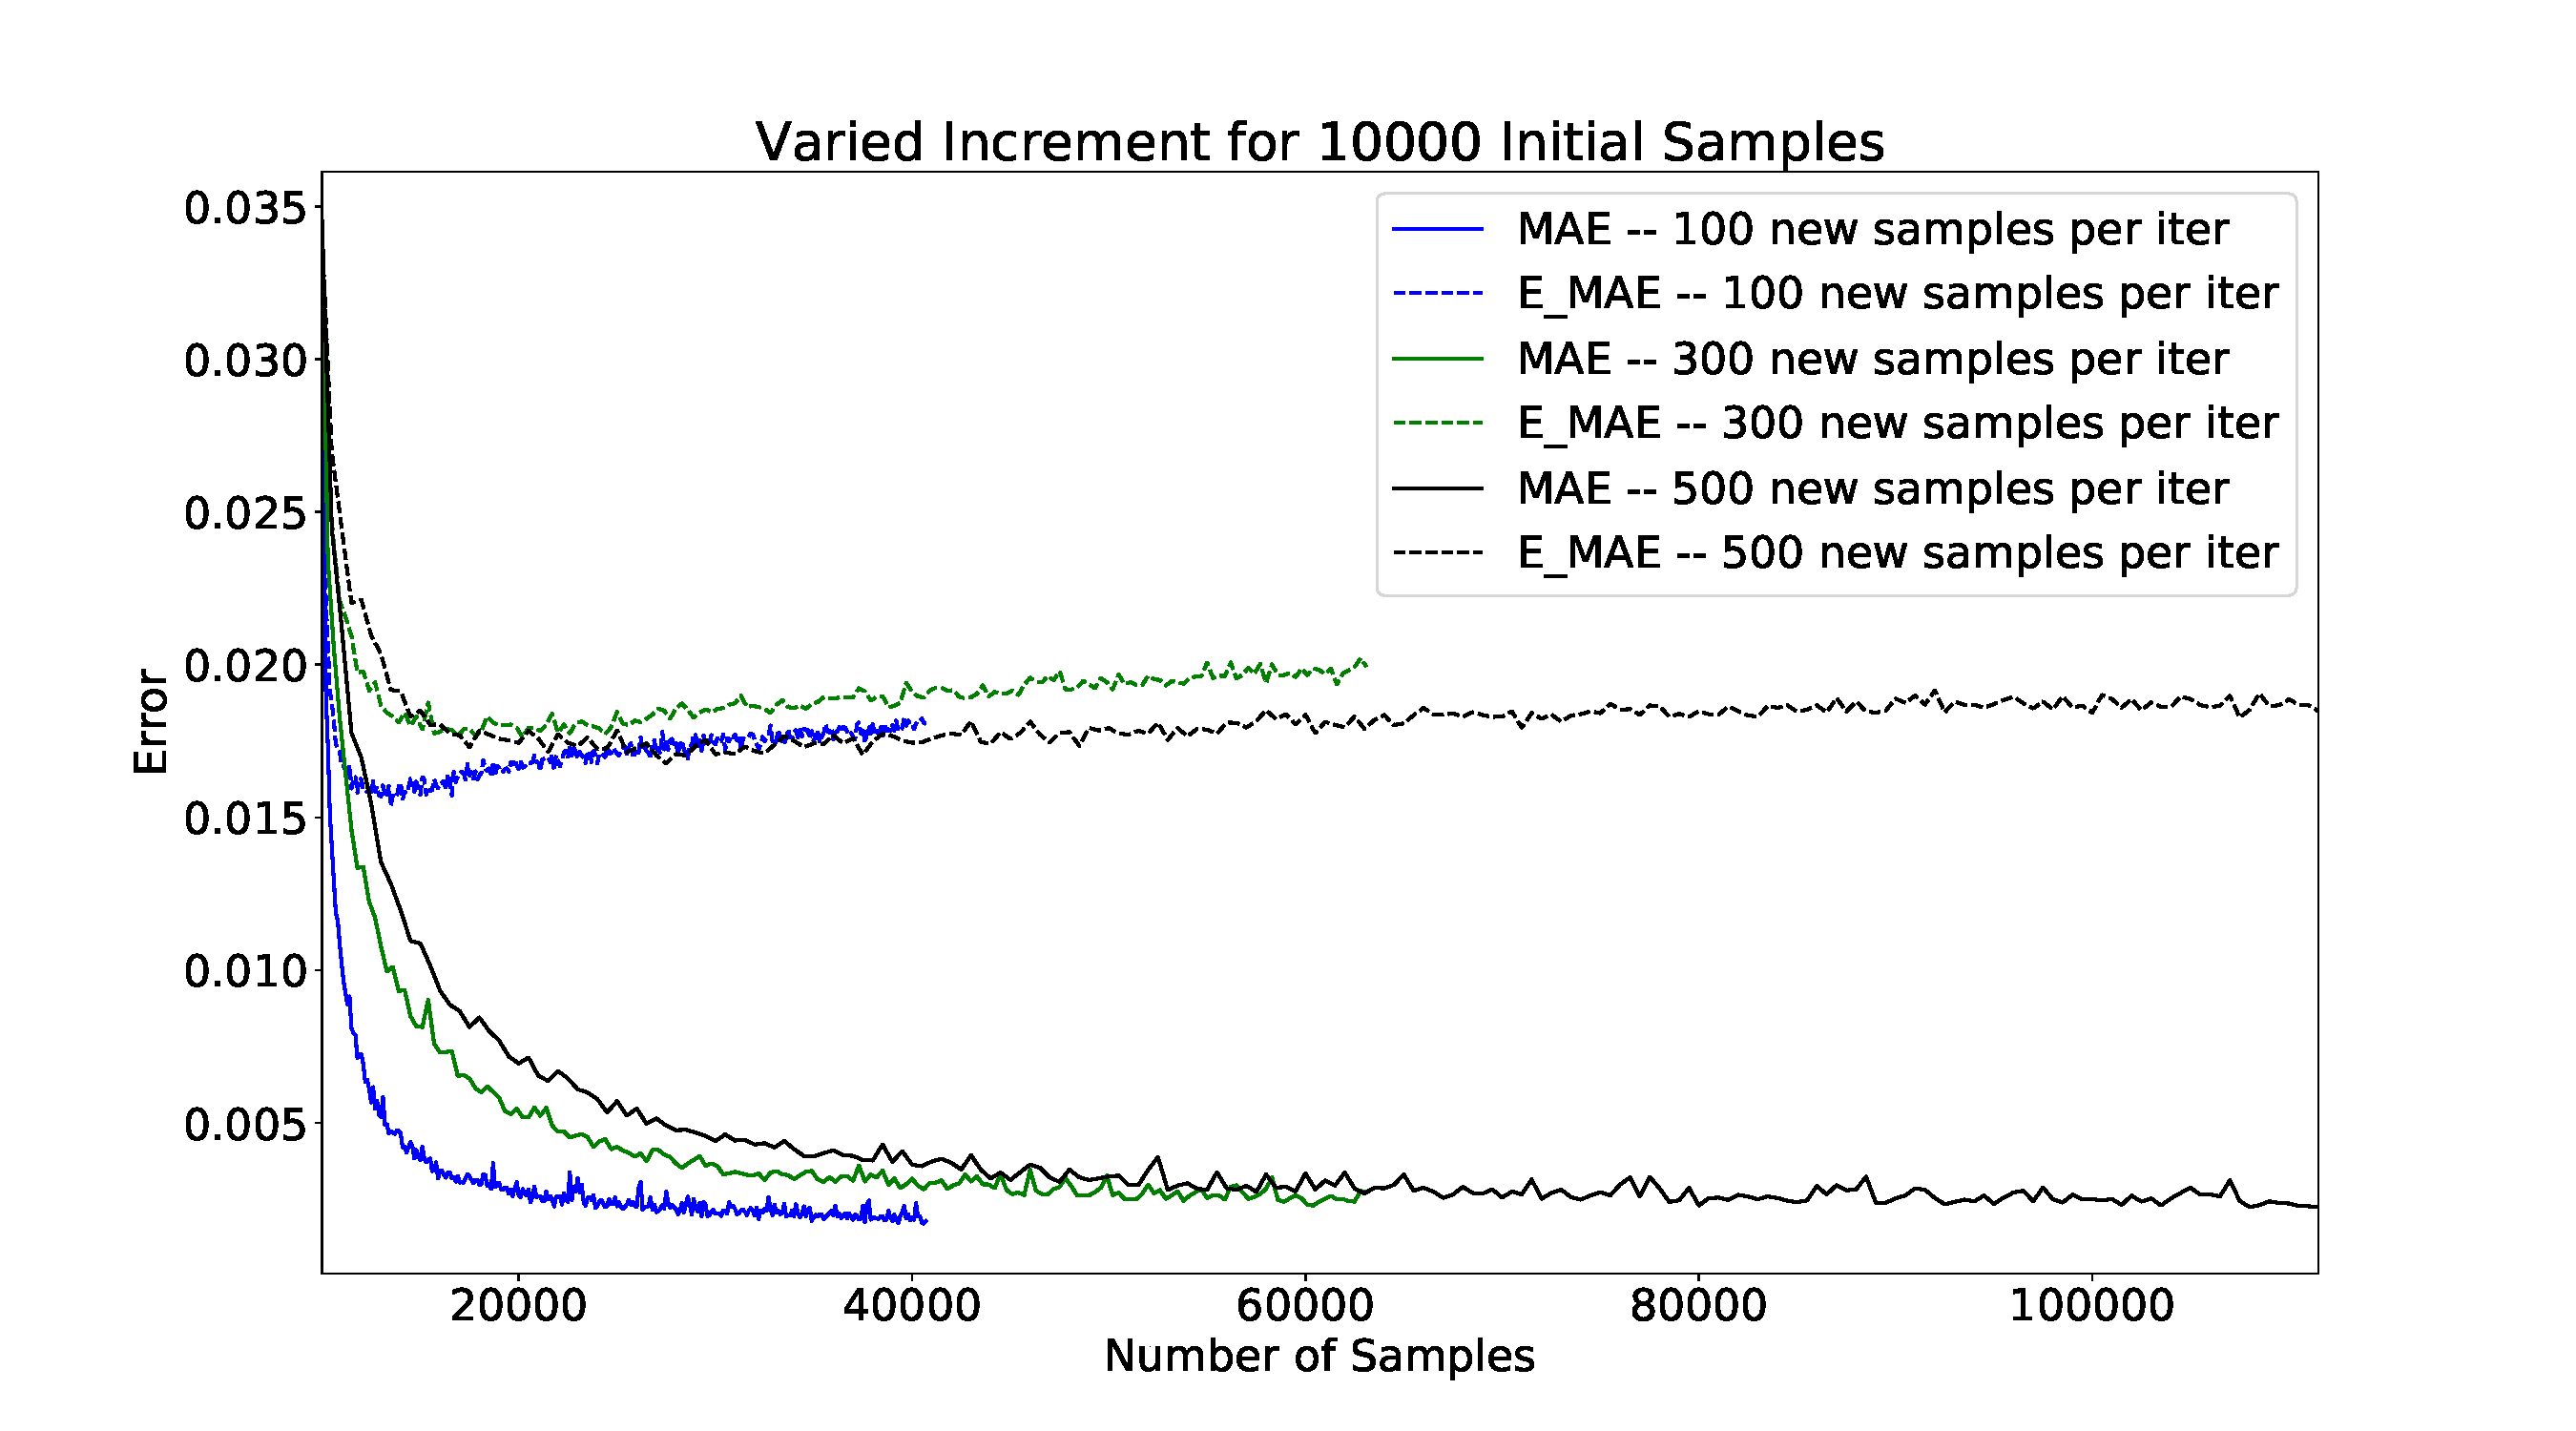
\includegraphics[width=1.1\linewidth]{fig6a_qassincrsamp.pdf}
    \end{subfigure}%
    ~ 
    \begin{subfigure}[t]{0.5\textwidth}
        \centering
        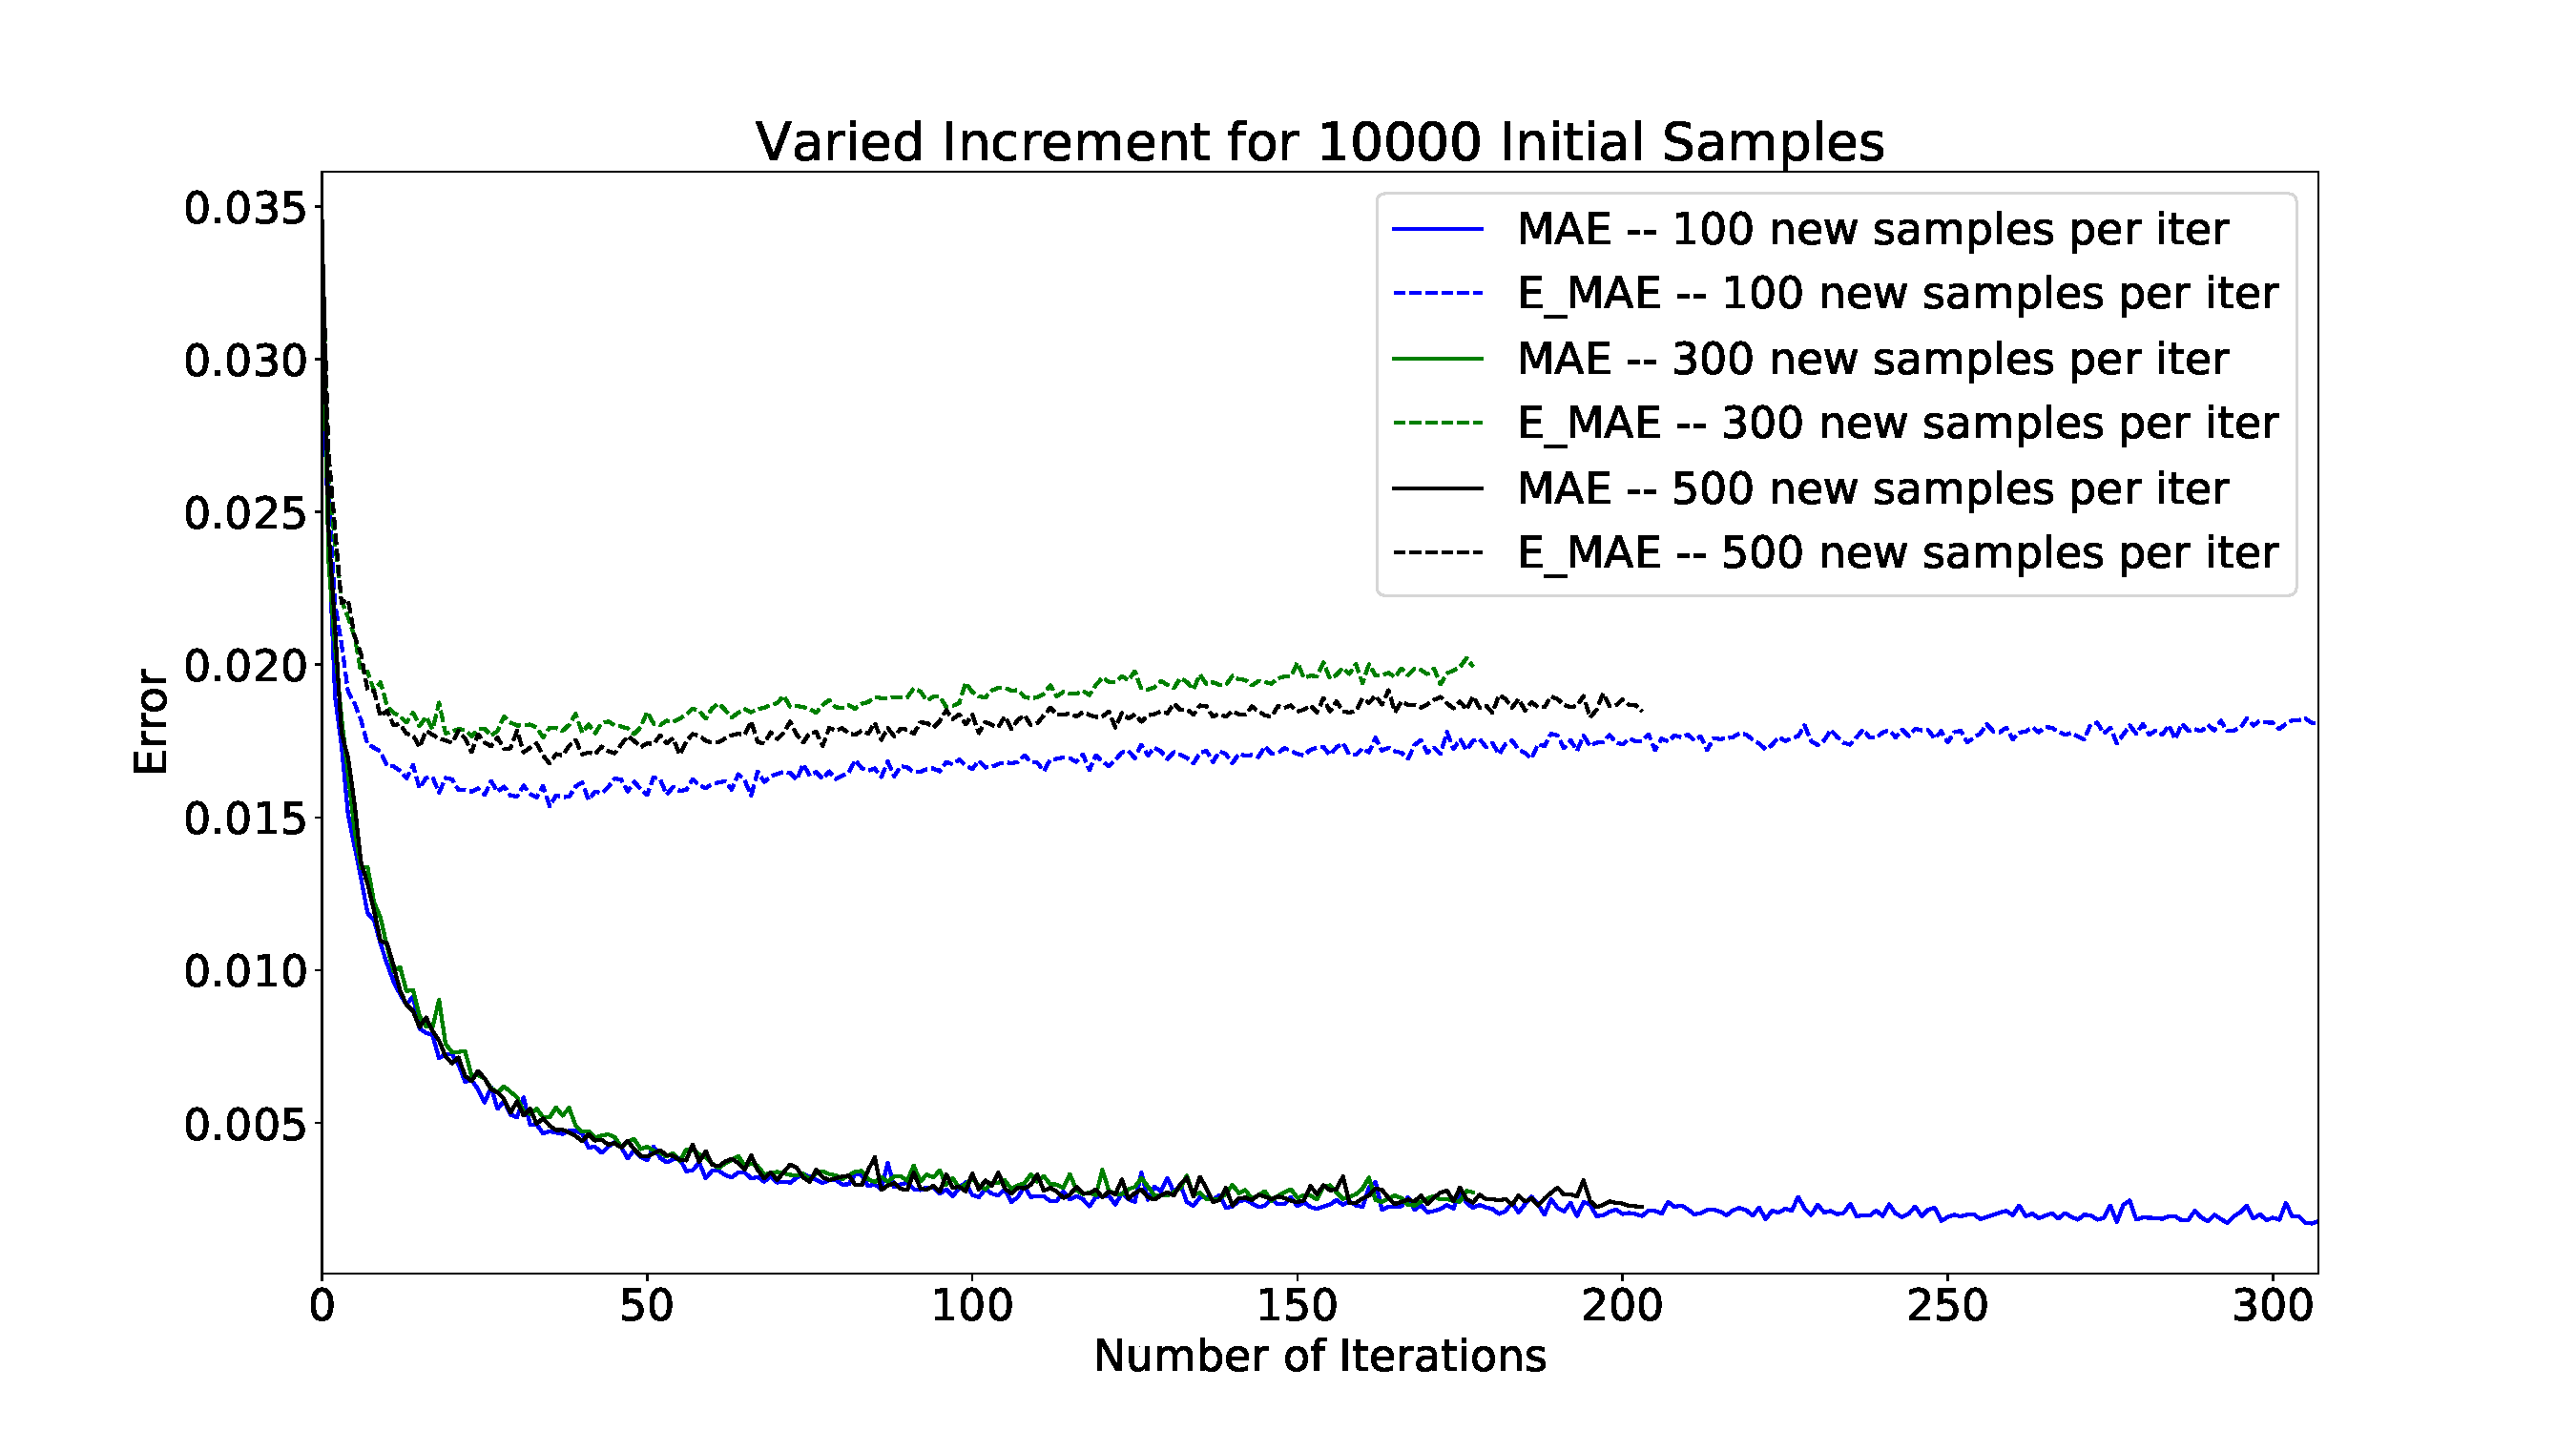
\includegraphics[width=1.1\linewidth]{fig6b_qassincrtime.pdf}
    \end{subfigure}
    \caption{QASS absolute training error over total sample quantity (left) and number of iterations (right). MAE represents surrogate error on the adaptively-sampled training/test set, and E\_MAE on the independent evaluation sets.}
    \label{fig:qassincr}
\end{figure}

The plateau effect in surrogate error on the evaluation set, seen
in~\cref{fig:qassincr}, was universal to all configurations and thought to
warrant further investigation. At first this was suspected to be a residual
effect of retraining the same ANN instance without adjustment to data
normalisation; a "Goldilocks scheme" for checking normalisation drift was
implemented and tested, but did not affect QASS performance. Schemes in which
the ANN is periodically retrained were also discarded, as the retention of
network weights from one iteration to the next was demonstrated to greatly
benefit QASS efficiency. Further insight came from direct comparison between
QASS and a baseline scheme with uniformly random incremental samples, shown
in~\cref{fig:qasssampling}.

\begin{figure}[h]
  \centering
    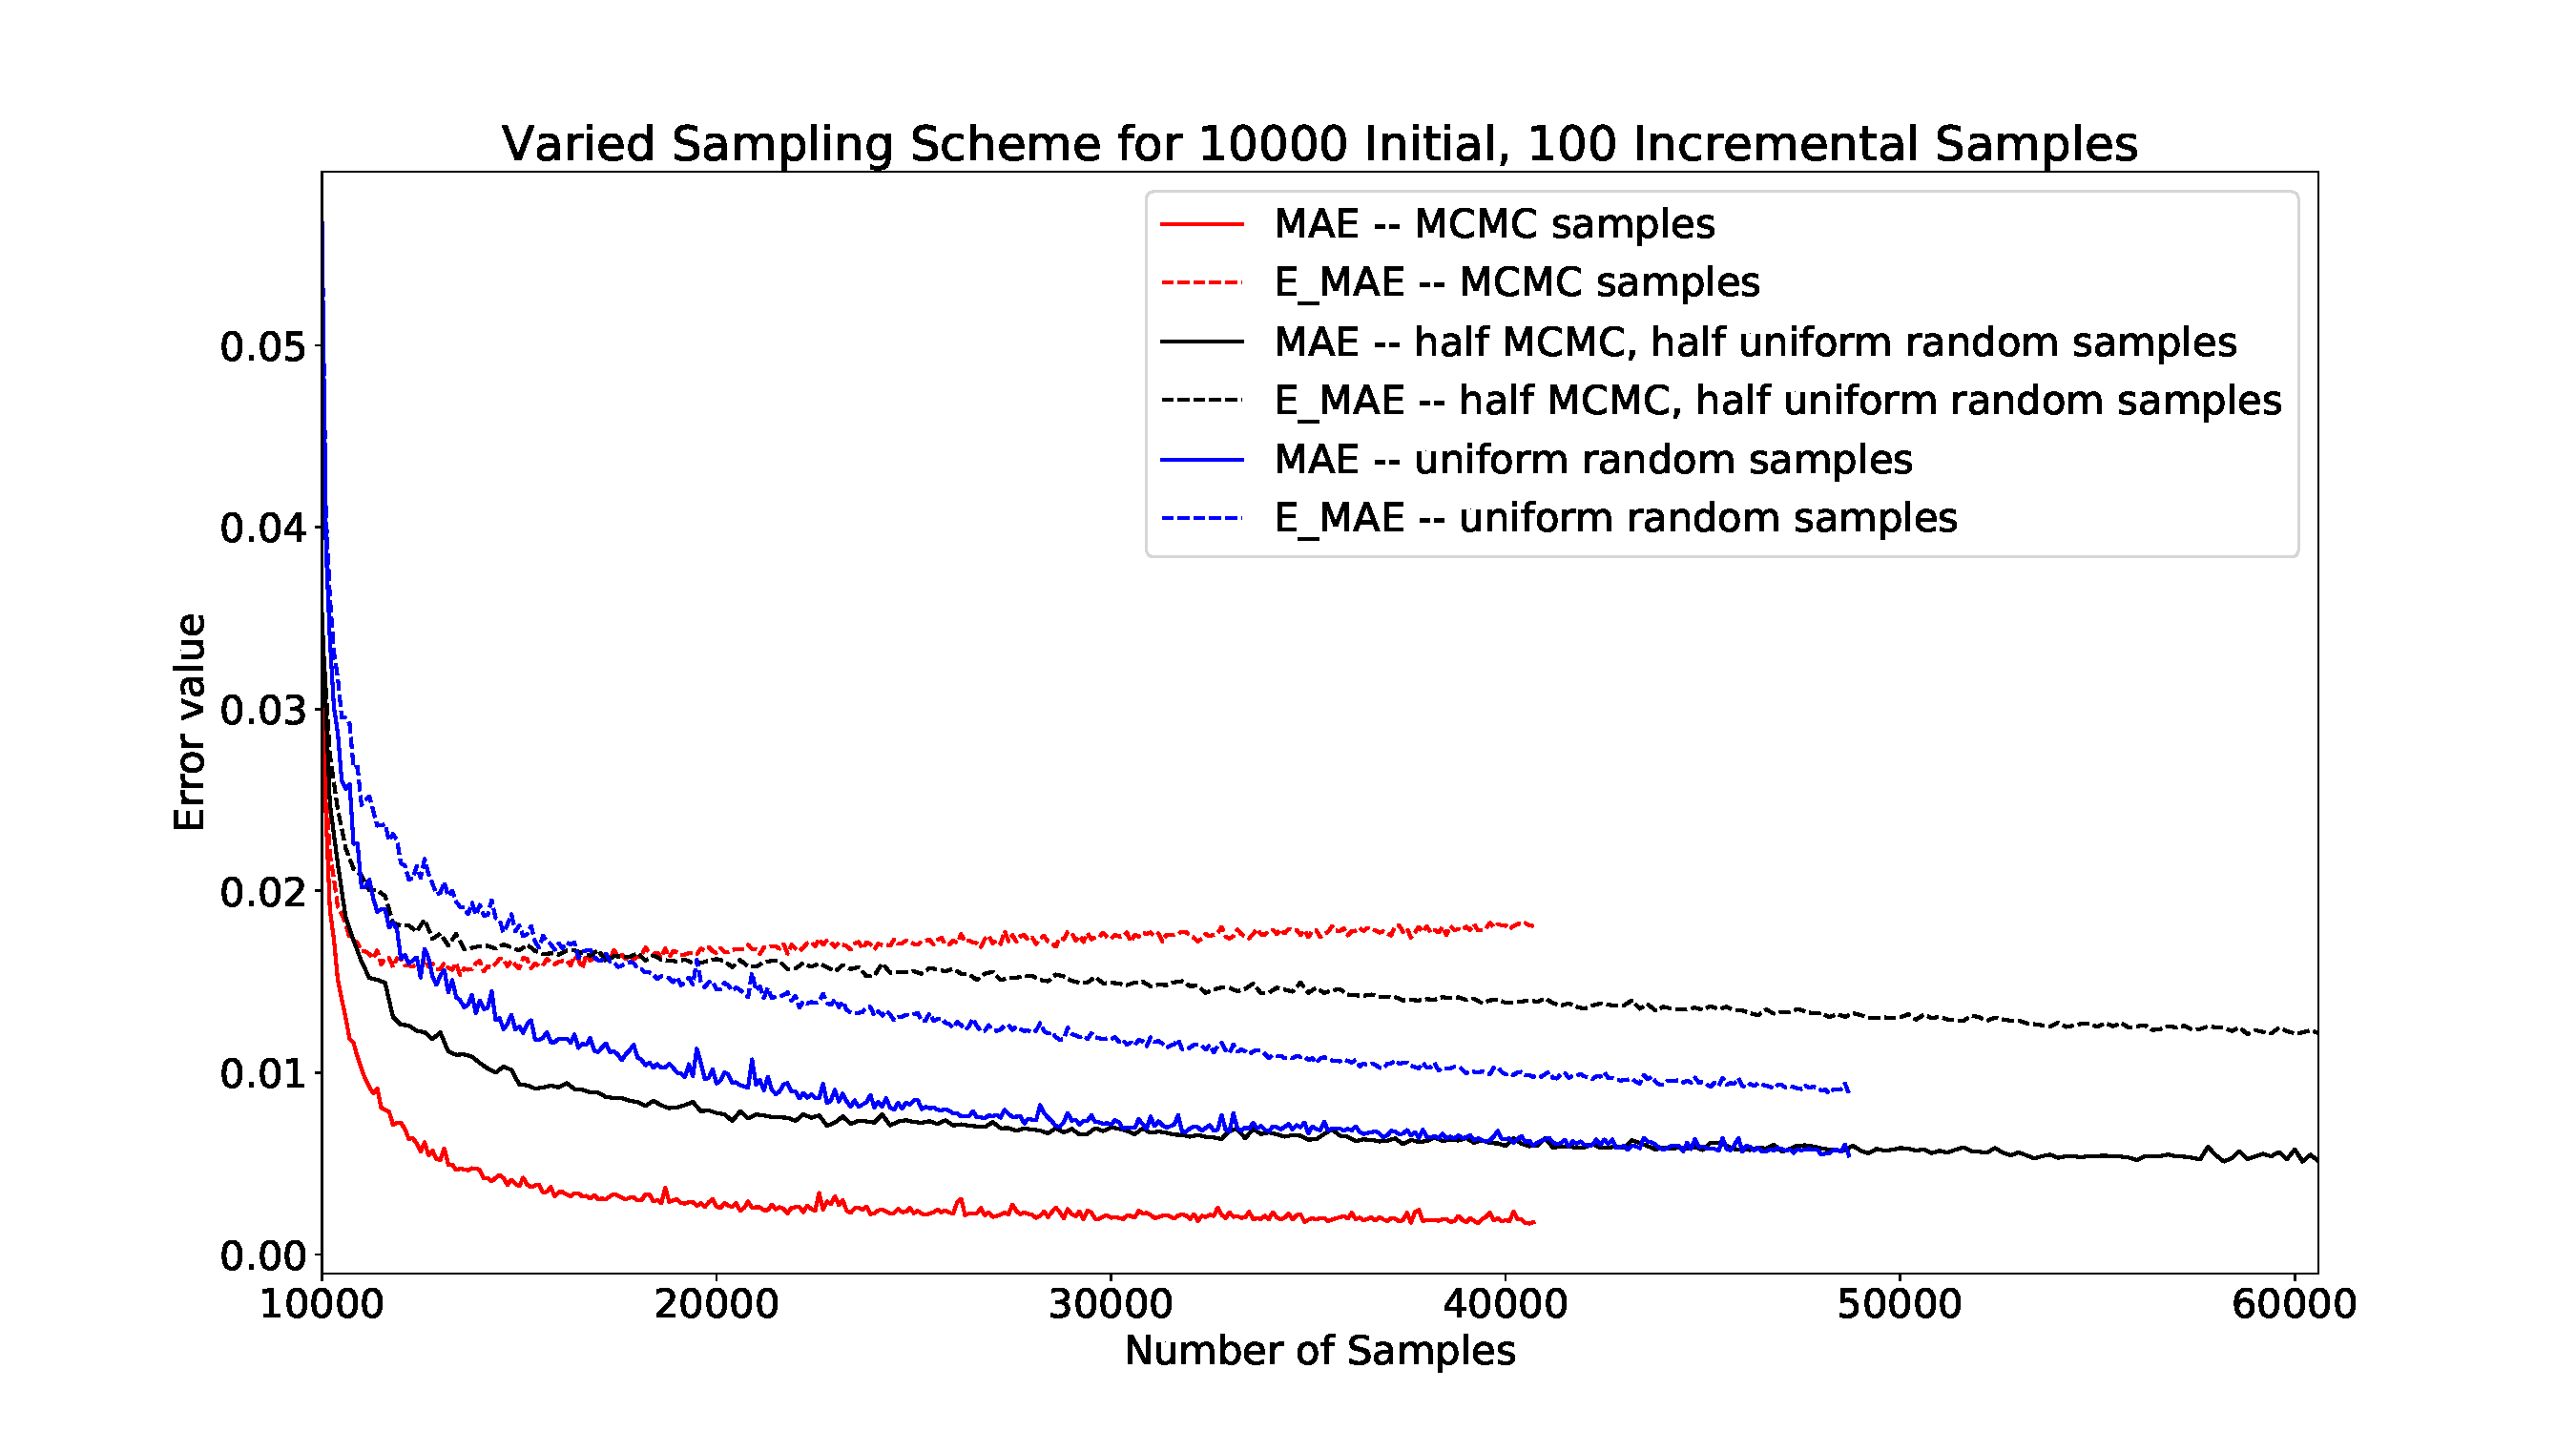
\includegraphics[width=0.8\linewidth]{fig7_qasssampling.pdf}
    \caption{Absolute training error for QASS, baseline scheme, and mixed scheme}
  \label{fig:qasssampling}
\end{figure}

Such tests revealed that while QASS has unmatched performance on its own
adaptively-sampled training set, it is outperformed by the baseline scheme on
uniformly random evaluation sets. We suspected that while QASS excels in
learning the most strongly peaked regions of the TBR theory, this comes at the
expense of precision in broader, smoother regions where uniformly random
sampling suffices. Therefore a mixed scheme was implemented, with half MCMC
samples and half uniformly random samples incremented on each iteration, which
is also shown in~\cref{fig:qasssampling}.
